% Options for packages loaded elsewhere
\PassOptionsToPackage{unicode}{hyperref}
\PassOptionsToPackage{hyphens}{url}
\PassOptionsToPackage{dvipsnames,svgnames,x11names}{xcolor}
%
\documentclass[
  letterpaper,
  DIV=11,
  numbers=noendperiod]{scrreprt}

\usepackage{amsmath,amssymb}
\usepackage{iftex}
\ifPDFTeX
  \usepackage[T1]{fontenc}
  \usepackage[utf8]{inputenc}
  \usepackage{textcomp} % provide euro and other symbols
\else % if luatex or xetex
  \usepackage{unicode-math}
  \defaultfontfeatures{Scale=MatchLowercase}
  \defaultfontfeatures[\rmfamily]{Ligatures=TeX,Scale=1}
\fi
\usepackage{lmodern}
\ifPDFTeX\else  
    % xetex/luatex font selection
\fi
% Use upquote if available, for straight quotes in verbatim environments
\IfFileExists{upquote.sty}{\usepackage{upquote}}{}
\IfFileExists{microtype.sty}{% use microtype if available
  \usepackage[]{microtype}
  \UseMicrotypeSet[protrusion]{basicmath} % disable protrusion for tt fonts
}{}
\makeatletter
\@ifundefined{KOMAClassName}{% if non-KOMA class
  \IfFileExists{parskip.sty}{%
    \usepackage{parskip}
  }{% else
    \setlength{\parindent}{0pt}
    \setlength{\parskip}{6pt plus 2pt minus 1pt}}
}{% if KOMA class
  \KOMAoptions{parskip=half}}
\makeatother
\usepackage{xcolor}
\setlength{\emergencystretch}{3em} % prevent overfull lines
\setcounter{secnumdepth}{5}
% Make \paragraph and \subparagraph free-standing
\makeatletter
\ifx\paragraph\undefined\else
  \let\oldparagraph\paragraph
  \renewcommand{\paragraph}{
    \@ifstar
      \xxxParagraphStar
      \xxxParagraphNoStar
  }
  \newcommand{\xxxParagraphStar}[1]{\oldparagraph*{#1}\mbox{}}
  \newcommand{\xxxParagraphNoStar}[1]{\oldparagraph{#1}\mbox{}}
\fi
\ifx\subparagraph\undefined\else
  \let\oldsubparagraph\subparagraph
  \renewcommand{\subparagraph}{
    \@ifstar
      \xxxSubParagraphStar
      \xxxSubParagraphNoStar
  }
  \newcommand{\xxxSubParagraphStar}[1]{\oldsubparagraph*{#1}\mbox{}}
  \newcommand{\xxxSubParagraphNoStar}[1]{\oldsubparagraph{#1}\mbox{}}
\fi
\makeatother

\usepackage{color}
\usepackage{fancyvrb}
\newcommand{\VerbBar}{|}
\newcommand{\VERB}{\Verb[commandchars=\\\{\}]}
\DefineVerbatimEnvironment{Highlighting}{Verbatim}{commandchars=\\\{\}}
% Add ',fontsize=\small' for more characters per line
\usepackage{framed}
\definecolor{shadecolor}{RGB}{241,243,245}
\newenvironment{Shaded}{\begin{snugshade}}{\end{snugshade}}
\newcommand{\AlertTok}[1]{\textcolor[rgb]{0.68,0.00,0.00}{#1}}
\newcommand{\AnnotationTok}[1]{\textcolor[rgb]{0.37,0.37,0.37}{#1}}
\newcommand{\AttributeTok}[1]{\textcolor[rgb]{0.40,0.45,0.13}{#1}}
\newcommand{\BaseNTok}[1]{\textcolor[rgb]{0.68,0.00,0.00}{#1}}
\newcommand{\BuiltInTok}[1]{\textcolor[rgb]{0.00,0.23,0.31}{#1}}
\newcommand{\CharTok}[1]{\textcolor[rgb]{0.13,0.47,0.30}{#1}}
\newcommand{\CommentTok}[1]{\textcolor[rgb]{0.37,0.37,0.37}{#1}}
\newcommand{\CommentVarTok}[1]{\textcolor[rgb]{0.37,0.37,0.37}{\textit{#1}}}
\newcommand{\ConstantTok}[1]{\textcolor[rgb]{0.56,0.35,0.01}{#1}}
\newcommand{\ControlFlowTok}[1]{\textcolor[rgb]{0.00,0.23,0.31}{\textbf{#1}}}
\newcommand{\DataTypeTok}[1]{\textcolor[rgb]{0.68,0.00,0.00}{#1}}
\newcommand{\DecValTok}[1]{\textcolor[rgb]{0.68,0.00,0.00}{#1}}
\newcommand{\DocumentationTok}[1]{\textcolor[rgb]{0.37,0.37,0.37}{\textit{#1}}}
\newcommand{\ErrorTok}[1]{\textcolor[rgb]{0.68,0.00,0.00}{#1}}
\newcommand{\ExtensionTok}[1]{\textcolor[rgb]{0.00,0.23,0.31}{#1}}
\newcommand{\FloatTok}[1]{\textcolor[rgb]{0.68,0.00,0.00}{#1}}
\newcommand{\FunctionTok}[1]{\textcolor[rgb]{0.28,0.35,0.67}{#1}}
\newcommand{\ImportTok}[1]{\textcolor[rgb]{0.00,0.46,0.62}{#1}}
\newcommand{\InformationTok}[1]{\textcolor[rgb]{0.37,0.37,0.37}{#1}}
\newcommand{\KeywordTok}[1]{\textcolor[rgb]{0.00,0.23,0.31}{\textbf{#1}}}
\newcommand{\NormalTok}[1]{\textcolor[rgb]{0.00,0.23,0.31}{#1}}
\newcommand{\OperatorTok}[1]{\textcolor[rgb]{0.37,0.37,0.37}{#1}}
\newcommand{\OtherTok}[1]{\textcolor[rgb]{0.00,0.23,0.31}{#1}}
\newcommand{\PreprocessorTok}[1]{\textcolor[rgb]{0.68,0.00,0.00}{#1}}
\newcommand{\RegionMarkerTok}[1]{\textcolor[rgb]{0.00,0.23,0.31}{#1}}
\newcommand{\SpecialCharTok}[1]{\textcolor[rgb]{0.37,0.37,0.37}{#1}}
\newcommand{\SpecialStringTok}[1]{\textcolor[rgb]{0.13,0.47,0.30}{#1}}
\newcommand{\StringTok}[1]{\textcolor[rgb]{0.13,0.47,0.30}{#1}}
\newcommand{\VariableTok}[1]{\textcolor[rgb]{0.07,0.07,0.07}{#1}}
\newcommand{\VerbatimStringTok}[1]{\textcolor[rgb]{0.13,0.47,0.30}{#1}}
\newcommand{\WarningTok}[1]{\textcolor[rgb]{0.37,0.37,0.37}{\textit{#1}}}

\providecommand{\tightlist}{%
  \setlength{\itemsep}{0pt}\setlength{\parskip}{0pt}}\usepackage{longtable,booktabs,array}
\usepackage{calc} % for calculating minipage widths
% Correct order of tables after \paragraph or \subparagraph
\usepackage{etoolbox}
\makeatletter
\patchcmd\longtable{\par}{\if@noskipsec\mbox{}\fi\par}{}{}
\makeatother
% Allow footnotes in longtable head/foot
\IfFileExists{footnotehyper.sty}{\usepackage{footnotehyper}}{\usepackage{footnote}}
\makesavenoteenv{longtable}
\usepackage{graphicx}
\makeatletter
\def\maxwidth{\ifdim\Gin@nat@width>\linewidth\linewidth\else\Gin@nat@width\fi}
\def\maxheight{\ifdim\Gin@nat@height>\textheight\textheight\else\Gin@nat@height\fi}
\makeatother
% Scale images if necessary, so that they will not overflow the page
% margins by default, and it is still possible to overwrite the defaults
% using explicit options in \includegraphics[width, height, ...]{}
\setkeys{Gin}{width=\maxwidth,height=\maxheight,keepaspectratio}
% Set default figure placement to htbp
\makeatletter
\def\fps@figure{htbp}
\makeatother
% definitions for citeproc citations
\NewDocumentCommand\citeproctext{}{}
\NewDocumentCommand\citeproc{mm}{%
  \begingroup\def\citeproctext{#2}\cite{#1}\endgroup}
\makeatletter
 % allow citations to break across lines
 \let\@cite@ofmt\@firstofone
 % avoid brackets around text for \cite:
 \def\@biblabel#1{}
 \def\@cite#1#2{{#1\if@tempswa , #2\fi}}
\makeatother
\newlength{\cslhangindent}
\setlength{\cslhangindent}{1.5em}
\newlength{\csllabelwidth}
\setlength{\csllabelwidth}{3em}
\newenvironment{CSLReferences}[2] % #1 hanging-indent, #2 entry-spacing
 {\begin{list}{}{%
  \setlength{\itemindent}{0pt}
  \setlength{\leftmargin}{0pt}
  \setlength{\parsep}{0pt}
  % turn on hanging indent if param 1 is 1
  \ifodd #1
   \setlength{\leftmargin}{\cslhangindent}
   \setlength{\itemindent}{-1\cslhangindent}
  \fi
  % set entry spacing
  \setlength{\itemsep}{#2\baselineskip}}}
 {\end{list}}
\usepackage{calc}
\newcommand{\CSLBlock}[1]{\hfill\break\parbox[t]{\linewidth}{\strut\ignorespaces#1\strut}}
\newcommand{\CSLLeftMargin}[1]{\parbox[t]{\csllabelwidth}{\strut#1\strut}}
\newcommand{\CSLRightInline}[1]{\parbox[t]{\linewidth - \csllabelwidth}{\strut#1\strut}}
\newcommand{\CSLIndent}[1]{\hspace{\cslhangindent}#1}

\KOMAoption{captions}{tableheading}
\makeatletter
\@ifpackageloaded{bookmark}{}{\usepackage{bookmark}}
\makeatother
\makeatletter
\@ifpackageloaded{caption}{}{\usepackage{caption}}
\AtBeginDocument{%
\ifdefined\contentsname
  \renewcommand*\contentsname{Tabla de contenidos}
\else
  \newcommand\contentsname{Tabla de contenidos}
\fi
\ifdefined\listfigurename
  \renewcommand*\listfigurename{Listado de Figuras}
\else
  \newcommand\listfigurename{Listado de Figuras}
\fi
\ifdefined\listtablename
  \renewcommand*\listtablename{Listado de Tablas}
\else
  \newcommand\listtablename{Listado de Tablas}
\fi
\ifdefined\figurename
  \renewcommand*\figurename{Figura}
\else
  \newcommand\figurename{Figura}
\fi
\ifdefined\tablename
  \renewcommand*\tablename{Tabla}
\else
  \newcommand\tablename{Tabla}
\fi
}
\@ifpackageloaded{float}{}{\usepackage{float}}
\floatstyle{ruled}
\@ifundefined{c@chapter}{\newfloat{codelisting}{h}{lop}}{\newfloat{codelisting}{h}{lop}[chapter]}
\floatname{codelisting}{Listado}
\newcommand*\listoflistings{\listof{codelisting}{Listado de Listados}}
\makeatother
\makeatletter
\makeatother
\makeatletter
\@ifpackageloaded{caption}{}{\usepackage{caption}}
\@ifpackageloaded{subcaption}{}{\usepackage{subcaption}}
\makeatother

\ifLuaTeX
\usepackage[bidi=basic]{babel}
\else
\usepackage[bidi=default]{babel}
\fi
\babelprovide[main,import]{spanish}
% get rid of language-specific shorthands (see #6817):
\let\LanguageShortHands\languageshorthands
\def\languageshorthands#1{}
\ifLuaTeX
  \usepackage{selnolig}  % disable illegal ligatures
\fi
\usepackage{bookmark}

\IfFileExists{xurl.sty}{\usepackage{xurl}}{} % add URL line breaks if available
\urlstyle{same} % disable monospaced font for URLs
\hypersetup{
  pdftitle={Bitácoras Grupo \#5, CA-204 (II-2024)},
  pdfauthor={Jeikel Navarro Solis, Gabriel Valverde, Erick Venegas},
  pdflang={es},
  colorlinks=true,
  linkcolor={blue},
  filecolor={Maroon},
  citecolor={Blue},
  urlcolor={Blue},
  pdfcreator={LaTeX via pandoc}}


\title{Bitácoras Grupo \#5, CA-204 (II-2024)}
\author{Jeikel Navarro Solis, Gabriel Valverde, Erick Venegas}
\date{2024-09-26}

\begin{document}
\maketitle

\renewcommand*\contentsname{Tabla de contenidos}
{
\hypersetup{linkcolor=}
\setcounter{tocdepth}{2}
\tableofcontents
}

\bookmarksetup{startatroot}

\chapter*{Introducción}\label{introducciuxf3n}
\addcontentsline{toc}{chapter}{Introducción}

\markboth{Introducción}{Introducción}

Este estudio utiliza una base de datos de riesgos financieros en el cual
se toman en cuanta variables como lo son la edad, genero, pais en el que
vive y estado marital de las personas, esto con el fin de realizar un
perfil descriptivo de los prestatario, asi como tambien se toman
variables cuantitativas como los ingresos, activos y deuda de la persona
en cuestion. De manera que la base contiene un total de 15000 casos y 20
variables. El objetivo es generar empiricamente un metodo que basado en
las variables permita crear una calificación de riesgo, tal que se
puedan relacionar las variables cuantitativas y cualitativas de modo tal
se logre llegar a algún resultado satisfactorio a partir de estos datos.
Por estas razones, la investigación se basa en un marco teorico y
empirico donde los autores buscan salir de la norma y explorar mas
factores que solo la parte economica de los prestatarios.

\bookmarksetup{startatroot}

\chapter{Bitacora 1}\label{bitacora-1}

\section{Parte de planificación}\label{parte-de-planificaciuxf3n}

\subsection{Definión de la idea}\label{definiuxf3n-de-la-idea}

La idea principal de este trabajo es analizar una tabla de datos y
extraer información de utilidad de ésta, recordemos que este trabajo es
acerca de un curso de herramientas de datos, por lo que el enfoque de
este es saber aplicar técnicas al estudio. Sin embargo, por fines
académicos, buscaremos relaciones entre las variables, haciendo usos de
las librerías que posee R, el cual será nuestro lenguaje de programación
y análisis de datos, con los que realizaremos el trabajo.

El tema es de interés, pues tenemos una base de datos con una cantidad
considerable de variables, que se prestan para hacer un análisis
exhaustivo. En adición, los datos que posee la base de datos son datos
financieros, que sin duda son de interés bajo el contexto de la carrera.
Al realizar un análisis previo de la bibliografía, observamos quela
información es realmente abundante, pues el tema de riesgos financieros
es un tópico de suma importancia para las empresas.

\subsection{Conceptualización de la
idea}\label{conceptualizaciuxf3n-de-la-idea}

``Verificar una relación entre la calificación de riesgo con las
variables Nivel de educación, Ingresos, Monto del préstamo''. De la
pregunta anterior, nos interesa conceptualizar dicha idea, por lo que,
buscando la definición de las palabras que conforman la idea, en la RAE,
encontramos lo siguiente:

\begin{itemize}
\item
  Relación: Conexión, correspondencia.
\item
  Nivel: Medida de una cantidad con referencia a una escala determinada.
\item
  Educación: Acción y efecto de educar, instrucción por medio de la
  acción docente.
\item
  Ingresos: Caudal que entra en poder de alguien, y que le es de cargo
  en las cuentas.
\item
  Calificación: Puntuación obtenida en un examen o en cualquier tipo de
  prueba.
\item
  Riesgo: Contingencia o proximidad de un daño.
\end{itemize}

\subsection{Identificación de
tensiones}\label{identificaciuxf3n-de-tensiones}

Como mencionamos en el apartado anterior, el trabajo se centra más en el
estudio de las herramientas utilizadas, que en la información del
trabajo per se. Sin embargo, vamos a desarrollar la teoría de manera
satisfactoria con el hecho de crear un trabajo bien estructurado. Dicho
lo anterior, es claro que la calificación de riesgo es un fenómeno que
depende de muchas más variables, un ejemplo de ello puede ser la cultura
de la sociedad en la cual se ve inmersa la persona que solicita el
préstamo, como la entidad que lo desembolsa. Por ello, el origen de los
datos de esta tabla de datos es de suma importancia, pues la cultura de
las personas que arrojaron estos datos puede influir de manera
sustancial en la salida de los datos.

Otro factor a tomar en cuenta es por supuesto, la tabla de datos, pues
podría contener información errónea, o datos que no estén correctamente
digitados, además de que la tabla de datos tiene que ser convertida a
información más trabajable, es decir, muchas de las variables son
categóricas, por lo que una conversión a datos de diferente especie,
podría provocar que haya errores en la nueva tabla que se va a
manipular.

\subsection{Reformulación de la idea en modo
preguntas}\label{reformulaciuxf3n-de-la-idea-en-modo-preguntas}

La idea principal de este trabajo es: ``Verificar una relación entre la
calificación de riesgo con las variables Nivel de educación, Ingresos,
Monto del préstamo'', por lo que para etsa parte del trabajo, vamos a
formular la idea de diferentes formas, esto con el fin de formular una
pregunta de investigación que sea clara.

\emph{¿Cuáles son las variables que influyen más en la calificación de
riesgo? }¿Existe una correlación positiva entre las variables de interés
y la calificación de riesgo? \emph{¿Es la calificación de riesgo un buen
calificador de las variables que la determinan? }¿Cómo se mide la
calificación de riesgo dadas las variables consideradas?

\subsection{Argumentación de las
preguntas}\label{argumentaciuxf3n-de-las-preguntas}

Estas preguntas deben poseer una argumentación detrás de ellas, pues es
necesario tener una idea de qué es lo que queremos realizar con estas
preguntas o dicho de otra forma, cuál es el problema que potencialmente
podemos resolver o la incógnita a contestar.8

\subsubsection{¿Cuáles son las variables que influyen más en la
calificación de
riesgo?}\label{cuuxe1les-son-las-variables-que-influyen-muxe1s-en-la-calificaciuxf3n-de-riesgo}

\textbf{Contraargumentos}

Las variables que se toman son realmente las correctas, cuál es el
método que se utiliza para determinar que las variables que se están
tomando son mejores para un resultado que otras. Al ser una calificación
de riesgo, que facilita el préstamo a personas o no, las personas
podrían tener intenciones perversas a siempre manipular su información
para obtener buenas calificaciones. Por otro lado, son muchas las
variables contempladas en la base de datos, hacer uso de un par de
variables, podría influir de manera considerable en buscar una relación
entre las variables.

\textbf{Argumentos}

Al realizar un análisis previo de la tabla de datos, podríamos
determinar cuáles son las variables con mayor impacto en esta
calificación, y así simplificar el modelo y darle un mayor énfasis en
estas variables que afectan de manera considerable en la calificación.

\textbf{Concluya}

Al ser una calificación de riesgo, las empresas deben considerar varios
factores, para ver si sus clientes son ideales para el préstamo o no.
Por otro lado, concentrarnos en las variables que tienen mayor peso,
podría ayudar a un mejor entendimiento de la calificación de riesgo.

\subsubsection{¿Existe una correlación positiva entre las variables de
interés y la calificación de
riesgo?}\label{existe-una-correlaciuxf3n-positiva-entre-las-variables-de-interuxe9s-y-la-calificaciuxf3n-de-riesgo}

\textbf{Contraargumentos} Una relación positiva no implica que haya una
mejor calificación, pues pueden existir variables con relación negativa,
que tengan un efecto positivo sobre la calificación de riesgo, por pura
intuición, podemos pensar en las personas que tienen un récord
crediticio limpio, esto implicaría que esta variable debería tener un
valor nulo para mejorar la calificación de riesgo. Otra variable que
podría afectar es las veces que la persona ha caído en impago, pues
entre más suba este valor, la calificación de riesgo, debería ser menor.

\textbf{Argumentos}

Las relaciones que buscamos no tienen por qué ser positivas, desde un
tipo de vista de coeficiente de correlación, sino desde un tipo de vista
de mejoría, es decir, variables que en ausencia contribuyan a una mejor
calificación, nos son de interés para el trabajo. Como hemos mencionado
encontrar las relaciones más contribuyentes, son de utilidad, pues
favorecen a simplificar el modelo y obtener a cambio una mejor
interpretación del estudio.

\textbf{Concluya}

Todas las relaciones son de importancia, hasta donde no existe relación,
pues sirven para delimitar el modelo y determinar cuáles son las
verdaderas variables que si influyen.

\subsubsection{\texorpdfstring{\textbf{¿Es la calificación de riesgo un
buen calificador de las variables que la
determinan?}}{¿Es la calificación de riesgo un buen calificador de las variables que la determinan?}}\label{es-la-calificaciuxf3n-de-riesgo-un-buen-calificador-de-las-variables-que-la-determinan}

\textbf{Contraargumentos}

Esta pregunta, no es del todo objetiva, pues dependerá de lo que la
empresa quiera detectar en estas evaluaciones, es decir, un factor que
determina en gran medida a la calificación de riesgo, en otra empresa no
tiene por qué ser así, pues dependerá del público objetivo de la
empresa. Un buen calificador de riesgo depende tanto de las variables
que se toman en cuenta, como del contexto de la empresa.

\textbf{Argumentos}

Desde el punto de vista de la empresa, la calificación de riesgo es una
herramienta que sirve para determinar en gran medida si un préstamo se
realiza o no, por ello, saber si su calificación de riesgo logra captar
la información deseada de las variables utilizadas, entonces se podría
considerar un buen factor, pues, aunque las empresas deban tener cuidado
a quiénes otorgan los préstamos, también es un hecho, que si no lo
hacen, se quedan sin negocio

\textbf{Concluya}

Si la calificación de riesgo logra simplificar y consolidar la
información, entonces podríamos conjeturar que se comporta como una
buena calificación.

\subsubsection{\texorpdfstring{\textbf{¿Cómo se mide la calificación de
riesgo dadas las variables
consideradas?}}{¿Cómo se mide la calificación de riesgo dadas las variables consideradas?}}\label{cuxf3mo-se-mide-la-calificaciuxf3n-de-riesgo-dadas-las-variables-consideradas}

\textbf{Contraargumentos}

La pregunta es más compleja que las hechas anteriormente, pues estamos
entrando a un método de calificación, es decir, hacer un análisis de la
medición, como mencionamos como un contraargumento en la pregunta
anterior, esto no tiene por qué ser universal en las empresas, esto
puede variar, por lo que dependerá del contexto en el cual se realice la
pregunta.

\textbf{Argumentos}

En realidad que sea una pregunta que depende de sus variables, podría
ser beneficioso, pues si existen varias metodologías, podríamos tener
una mejor cartera de préstamos, es decir, dado cierto tipo de cliente,
se podrían realizar cierto tipo de préstamos.

\textbf{Concluya}

La subjetividad de esta pregunta, no es ni buena ni mala, esta depende
su contexto, si es aplicada de una buena forma, podría ser beneficioso
tanto para la empresa, por ampliar su mercado, como para el cliente, al
recibir el préstamo deseado.

\subsection{Argumentación a través de
datos}\label{argumentaciuxf3n-a-travuxe9s-de-datos}

La base de datos utilizada en este trabajo se toma de la base de datos
de Kaggle. Sin embargo, el autor de la base de datos no publica la
información de cuándo es sacada la información. La información fue de
fácil acceso pues está disponible en la de datos de Kaggle. La muestra
observada son personas entre las edades de 18 a 69 años, de donde toman
muchas variables, las cuales veremos más adelante. La unidad estadística
estudiada para este trabajo son individuos que buscan obtener un
préstamo.

Para la siguiente vamos a tomar el nombre las variables, las cuales
dejaremos en el idioma original y vamos a dar la descripción de ellas,
las cuales viene a su vez con la tabla de datos.

\begin{itemize}
\item
  Age: La edad del individuo, una variable continua que influye en la
  estabilidad financiera.
\item
  Gender: Género del individuo, categorizado en Masculino, Femenino y No
  binario.
\item
  Education Level: Nivel de educación alcanzado, que varía desde la
  Secundaria hasta el Doctorado.
\item
  Marital Status: Estado civil actual, categorizado como Soltero,
  Casado, Divorciado o Viudo.
\item
  Income: Ingreso anual en USD, que representa la capacidad de ganancia
  del individuo.
\item
  Credit Score: Valor numérico que indica la solvencia crediticia, que
  varía de 600 a 800.
\item
  Loan Amount: La cantidad de préstamo solicitada por el individuo, que
  representa las necesidades financieras.
\item
  Loan Purpose: El propósito del préstamo, categorizado en Vivienda,
  Auto, Personal o Negocios.
\item
  Employment Status: Situación laboral del individuo, incluyendo
  Empleado, Desempleado o Autónomo.
\item
  Years at Current Job: Duración del empleo en el trabajo actual, que
  refleja la estabilidad laboral.
\item
  Payment History: Desempeño histórico de pagos, categorizado como
  Excelente, Bueno, Regular o Malo.
\item
  Debt-to-Income Ratio: Relación entre deuda e ingreso, que indica el
  apalancamiento financiero y el riesgo.
\item
  Assets Value: Valor total de los activos poseídos por el individuo.
\item
  Number of Dependents: Número de dependientes a cargo del individuo,
  que afecta las responsabilidades financieras.
\item
  City: Ciudad en la que reside el individuo, proporcionando contexto
  geográfico.
\item
  State: Estado en el que reside el individuo, proporcionando más
  detalles geográficos.
\item
  Country: País de residencia, añadiendo una perspectiva global.
\item
  Previous Defaults: Número de incumplimientos de préstamos anteriores,
  indicando el riesgo financiero histórico.
\item
  Marital Status: Número de cambios en el estado civil, reflejando
  cambios en la vida personal.
\item
  Risk Rating: Columna objetivo que categoriza el riesgo financiero en
  Bajo, Medio o Alto.
\end{itemize}

\section{Revisión bibliográfica}\label{revisiuxf3n-bibliogruxe1fica}

\subsection{Búsqueda de
bibliografía}\label{buxfasqueda-de-bibliografuxeda}

Entre las posibles combinaciones de palabras clave se se pueden
encontrar:

\begin{itemize}
\item
  Ingreso + situación laboral + solvencia crediticia
\item
  Prestamo + incumplimiento de préstamos + riesgo financiero
\item
  Ciudad + propósito del prestamo + ingreso
\item
  Situacion laboral + duración de empleo + historico de pagos
\item
  Historico de pagos + incumplimiento de prestamos + categoria de riesgo
\item
  Valor de activos + prestamo + relación entre deuda e ingreso
\end{itemize}

\subsection{Fichas de literatura}\label{fichas-de-literatura}

\textbf{Título: La valoración del riesgo financiero.}

\begin{itemize}
\item
  Autor: Dorina Chicu.
\item
  Año: 2020.
\item
  Nombre del tema: Métodos para medir el riesgo.
\item
  Cronología: 2020.
\item
  Metodología: Recolección de datos.
\item
  Temática: Estudios económicos.
\item
  Teórica: Valoración de riesgos.
\item
  Resumen en una oración: Distintos riesgos existentes y algunas formas
  de medirlos.
\item
  Argumento central: Analizar algunos de los distintos métodos
  existentes para medir los riesgos financieros.
\item
  Problema con el argumento o el tema: Aunque el tema principal gire en
  torno a la valoración de riesgos financieros, el trabajo queda falente
  de varios detalles que, si pudieran ser notorios a la hora de hacer un
  análisis más exhaustivo, además de la falta de ejemplos u aplicaciones
  de estos, quedan solo como algo teórico.
\item
  Resumen en un párrafo: El estudio busca centrarse en uno de los tres
  componentes de la inversión el cual es el riesgo financiero, de manera
  que se sabe que el objetivo principal de una empresa es maximizar sus
  beneficios, tal que llegue a asegurar la máxima rentabilidad posible.
  Por tanto, lo que se quiere brindar son los distintos métodos
  existentes que sirven para medir o valorar el riesgo, lo cual lleva a
  que sea posible generar una estrategia que permita mitigar los mismos.
\end{itemize}

\textbf{Título: La evaluación del riesgo de crédito en las instituciones
de microfinanzas: estado del arte. }

\begin{itemize}
\item
  Autor: María Seijas, Milagro Vivel, Rubén Lado, Sara Fernández.
\item
  Año: 2017.
\item
  Nombre del tema: Riesgos en los microcréditos.
\item
  Cronología: 2015 - 2017.
\item
  Metodología: Recolección y comparación de datos.
\item
  Temática: Estudios económicos.
\item
  Teórica: Valoración de riesgos.
\item
  Resumen en una oración: medición del riesgo de los microcréditos y
  análisis de los clientes.
\item
  Argumento central: Explorar la diversa teoría existente al riesgo de
  crédito de las instituciones financieras.
\item
  Problema con el argumento o el tema: Aunque el tema principal gire en
  torno a la valoración de riesgos financieros, el trabajo queda falente
  de varios detalles que, si pudieran ser notorios a la hora de hacer un
  análisis más exhaustivo, además de la falta de ejemplos u aplicaciones
  de estos, quedan solo como algo teórico.
\item
  Resumen en un párrafo: Este trabajo busca exponer a través de las
  investigaciones que se han centrado en la evaluación del riesgo de
  crédito en las Instituciones de Microfinanzas, aquella teoría
  relacionada con el riesgo presente en los microcréditos, además busca
  analizar todos aquellos factores que llegan a ser determinantes en el
  riesgo de que haya algún tipo de impago., por lo que este estudio
  también ofrece ciertas técnicas que generan una mayor consistencia y
  trasparencia en la evaluación y seguimiento de los clientes y su
  perfil.
\end{itemize}

\section{Construcción de la UVE de
Gowin}\label{construcciuxf3n-de-la-uve-de-gowin}

\begin{figure}[H]

{\centering 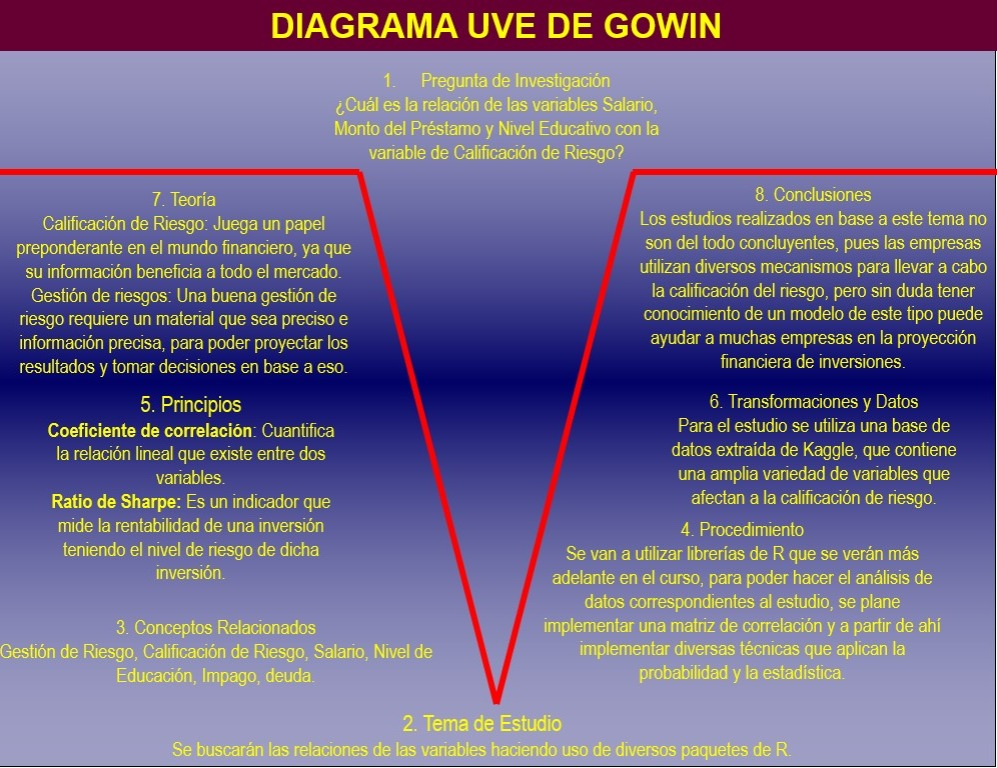
\includegraphics{imagenes/v-gowin.jpeg}

}

\caption{V de Gowin}

\end{figure}%

\subsection{Conceptos básicos}\label{conceptos-buxe1sicos}

Como hemos estado hablando a lo largo del trabajo, la calificación de
riesgo es de suma importancia, por lo que el estudio posee como objetivo
determinar una relación fuerte de las variables, para aproximar un
método empírico de una calificación de riesgo, pues ya vimos que las
empresas por lo general no comparten esta información.

Por otro lado, la gestión de riesgo y la incertidumbre se vuelven
esenciales a lo largo del trabajo, pues son conceptos que son base para
el estudio posterior. El riesgo de impago también se vuelve un concepto
a tener en cuenta, el cual vamos a entender como la incapacidad de
cumplir una obligación financiera.

\subsection{Principios y teorías}\label{principios-y-teoruxedas}

Para llevar a cabo la investigación en estas etapas preliminares hemos
hecho estudio bibliográfico de lo que son los análisis de calificación
financiera, que es justo el tema y variable objetivo de nuestro estudio.
También se incorpora la teoría de la gestión de riesgos, que a su vez
hace uso de técnicas de probabilidad pues dentro de su corpus la idea
principal es maximizar una ganancia en eventos que presentan
incertidumbre, de ahí la estrecha relación que tiene con Probabilidad.

Por otro lado, utilizar los conceptos de la valoración de riesgos
financieros, sirve de base para entender cómo funciona el mercado
financiero, y cuáles son los impactos directos de poseer una
calificación de riesgos, y que el impacto es de hecho, para todos los
participantes.

\section{Parte de escritura}\label{parte-de-escritura}

El problema que se va a tratar en el presente trabajo es de determinar
la relación existente entre las variables de ingresos, nivel de
educación y Monto del préstamo con la calificación de riesgo. Desde el
punto de vista teórico, el autor (Palacios 2012), menciona que ``La
principal función que radica en las calificaciones crediticias es la
evaluación de la mayor o menor probabilidad de pago de la deuda y los
intereses, proporcionando indicadores que sirvan de referencia a los
inversores con el fin de que puedan tener conocimiento del riesgo
crediticio de una forma simple y accesible''. Desde este punto de vista,
hay un apoyo en la investigación que tratamos de realizar, pues la
calificación de riesgo es de suma importancia en el mundo financiero.
Este mismo autor menciona que ``Su importancia deriva de su implantación
dentro de la regulación, lo que afecta a todo el entramado
institucional, y sectores clave de la sociedad como son el bancario y
las agencias de seguros y reaseguros'', podemos ver entonces que la
teoría respalda la importancia que hemos estado conjeturando en esta
presente bitácora (Entiéndase conjeturando, porque aún no hemos
realizado el análisis de la tabla de datos).

El estudio del análisis financiero es de suma importancia en la
actualidad, ya que las transacciones de los flujos de dinero cada vez
son mayores, es decir, vender deuda para obtener financiamiento en el
corto plazo es una de las estrategias más aplicadas, por ello tanto
inversores como prestatarios, según (Palacios 2012), ``Los inversores
hacen uso de las calificaciones crediticias como un indicador de la
probabilidad de recuperar su dinero. Adicionalmente, los prestatarios
pueden beneficiarse de tener calificada su deuda, con el objetivo de
colocarla con mayor facilidad y eliminar las dudas que haya relación a
ellos.'' Por ello, ambas parten obtienen beneficio de que exista este
rating en el mundo de la información financiera. Y desde el punto de
vista del inversor, como menciona la autora (Chicu 2020), ``\ldots a la
hora de analizar una inversión, debemos valorar la rentabilidad
esperada, así como la liquidez que perdemos y el riesgo que estamos
dispuestos a sumir''. Por lo tanto, poseer la información de rating es
de suma utilidad, pues ayuda a los inversores a realizar mejores
proyecciones. En adición, haciendo referencia a esta misma autora
``\ldots la gestión de riesgos tiene un lugar cada vez que un inversor
analiza e intenta cuantificar las pérdidas potenciales en una inversión
y luego toma las medidas apropiadas, considerando sus objetivos de
inversión y su tolerancia al riesgo.'' Esto último viene de la mano con
lo que son las proyecciones, pues le permite al inversionista hacer un
mejor análisis y una gestión de riesgos adecuada, que podemos definir
según Chicu como ``El proceso de identificación, análisis e
incorporación de la incertidumbre en las decisiones de inversión''
(Chicu 2020). Reforzando lo que menciona Chicu, la autora (Maria de los
Ángeles Herrera 2024), menciona en adición a la gestión de riesgos ``el
contexto de incertidumbre genera inevitablemente un riesgo, y es ahí
cuando la institución financiera debe preservar su valor económico y la
integridad de los recursos confiados por los depositantes y socios.'' Y
añadiendo la definición de esta misma autora tenemos que la gestión de
riesgos es ``la denominación que se utiliza para el conjunto de técnicas
y herramientas que pretenden maximizar el valor económico de la
institución financiera, en un contexto de incertidumbre''. Concluyendo,
la gestión de riesgos depende íntimamente de la calificación de riesgo,
pues permite tener un parámetro ante la incertidumbre que representa
invertir.

\section{Referencias bibliográfica}\label{referencias-bibliogruxe1fica}

\phantomsection\label{refs}
\begin{CSLReferences}{1}{0}
\bibitem[\citeproctext]{ref-chicu2020}
Chicu, Dorina. 2020. {«La valoración del riesgo financiero»}. 2020.
\url{https://openaccess.uoc.edu/bitstream/10609/150126/1/LaValoracionDelRiesgoFinanciero.pdf}.

\bibitem[\citeproctext]{ref-herrera2008}
Maria de los Ángeles Herrera, Juan Terán. 2024. {«Conceptualización del
riesgo de los mercados financieros»}. 2024.
\url{https://www.redalyc.org/pdf/900/90075920006.pdf}.

\bibitem[\citeproctext]{ref-palacios2012}
Palacios, Alberto. 2012. {«Calificación de riesgo: definición e
influencia en la última década»}. 2012.
\url{https://digibuo.uniovi.es/dspace/bitstream/handle/10651/4017/ACC-.pdf;jsessionid=723581A47435AFB6D2FEC05A70379F77?sequence=1}.

\end{CSLReferences}

\section{Anexo 1 (CHANGELOG)}\label{anexo-1-changelog}

\subsection{Chore}\label{chore}

\begin{itemize}
\tightlist
\item
  Agrega archivo configuracion pre-commit
\item
  Agrega configuracion repo-actions
\item
  Agrega cambios en docs/
\item
  Modifica la carpeta docs
\item
  Modifica la carpeta docs
\item
  Modifica la carpeta docs
\end{itemize}

\subsection{Feat}\label{feat}

\begin{itemize}
\tightlist
\item
  Agrega documentos para quarto
\item
  Agrega carpeta docs
\item
  Agrego la base de datos en formato csv
\item
  Agrego la base de datos en formato txt a manera de respaldo del
  archivo en formato csv. Cualquier cambio realizado al archivo original
  sera realizado en este tambien.
\item
  Agrega documentos Bitacora\_1
\item
  Agrega comentario en Bitacora\_1
\item
  Elimina la base de datos
\item
  Agrega la base de datos
\item
  Agrega la definición de la idea
\item
  Agrega en bitácora 1 identificación de tensiones
\item
  Agrega en bitácora 1, identificación de Tensiones
\item
  Agrega en bitácora 1, Reformulación de la idea en modo pregunta
\item
  Agrega en bitácora 1, argumentación de las preguntas
\item
  Agrega en bitácora 1, argumentación a través de datos
\item
  Agrega en Bitacora 1 avance de revisión bibliografica
\item
  Agrega en bitácora 1, parte de escritura
\item
  Agrega el archivo de references.bib
\item
  Agrega las referencias bibliograficas
\item
  Agrega en bitacora 1 principios y teorias
\item
  Agrega en bitacora 1 busqueda bibliografica
\item
  Agrega la introduccion
\item
  Se agrega a bitácora 1, la UVE de Gowin
\item
  Agrega imagen de la V de Gowin
\end{itemize}

\subsection{Fix}\label{fix}

\begin{itemize}
\tightlist
\item
  Arregla una funcionalidad de .gitignore
\item
  Corrige la numeración de la bitacora 1
\item
  Arreglo de index
\item
  Realiza correciones diversas en los documentos
\item
  Corrige error ortografico
\end{itemize}

\section{Anexo 2 (Participacion)}\label{anexo-2-participacion}

Puedes descargar el resumen de cambios \href{resumen.txt}{aquí}.

\bookmarksetup{startatroot}

\chapter{Bitácora 2}\label{bituxe1cora-2}

\section{Parte de Planificación}\label{parte-de-planificaciuxf3n-1}

\subsection{Ordenamiento de la
Literatura}\label{ordenamiento-de-la-literatura}

\section{Enlaces de la Literatura}\label{enlaces-de-la-literatura}

\section{Análisis Estadístico}\label{anuxe1lisis-estaduxedstico}

Como base para realizar este análisis estadístico, nos estamos guíando
con la guía del curso de Herramientas de Ciencias de Datos, el cual
adjuntamos el link a dicha guía https://maikolsolis.com/libros/hpcd/ y
también estamos utilizando el libro escrito por Wickham, el cual también
adjuntamos el link https://r4ds.hadley.nz/.

A modo de introducción, el análisis estadístico consiste en un conjunto
de herramientas o técnias que se utilizan para la recolección, el
análisis e interpretación de datos. Para este trabajo es imprescindible
contar con este set de herramientas.

\subsection{Análisis Descriptivo}\label{anuxe1lisis-descriptivo}

La base de datos ya se encuentra en formato en tidy, recordemos que el
formato tidy fue popularizado por el autor Hadley Wickham, donde indican
que cada variable debe tener su propia columna y cada observación su
propia fila. Nuestra base de datos cumple con estar en formato tidy.

Vamos a llamar a nuestra base de datos, la cual vamos a utilizar durante
el trabajo.

\begin{Shaded}
\begin{Highlighting}[]
\FunctionTok{library}\NormalTok{(readr)}
\NormalTok{base\_financial\_risk\_assessment }\OtherTok{\textless{}{-}} \FunctionTok{read\_delim}\NormalTok{(}\StringTok{"base{-}financial{-}risk{-}assessment.csv"}\NormalTok{, }
    \AttributeTok{delim =} \StringTok{";"}\NormalTok{, }\AttributeTok{escape\_double =} \ConstantTok{FALSE}\NormalTok{, }\AttributeTok{trim\_ws =} \ConstantTok{TRUE}\NormalTok{)}
\end{Highlighting}
\end{Shaded}

\begin{verbatim}
Rows: 15000 Columns: 20
-- Column specification --------------------------------------------------------
Delimiter: ";"
chr (10): Gender, Education Level, Marital Status, Loan Purpose, Employment ...
dbl (10): Age, Income, Credit Score, Loan Amount, Years at Current Job, Debt...

i Use `spec()` to retrieve the full column specification for this data.
i Specify the column types or set `show_col_types = FALSE` to quiet this message.
\end{verbatim}

\begin{Shaded}
\begin{Highlighting}[]
\FunctionTok{View}\NormalTok{(base\_financial\_risk\_assessment)}
\end{Highlighting}
\end{Shaded}

\begin{Shaded}
\begin{Highlighting}[]
\FunctionTok{View}\NormalTok{(base\_financial\_risk\_assessment)}
\end{Highlighting}
\end{Shaded}





\end{document}
